%%%%%%%%%%%%%%%%%%%%%%%%%%%%%%%%%%%%%%%%%%%%%%%%%%%%%%%%%%%%%%%%%%%%%%%%%%%%%%%
%% Copyright (c) 2010, 2020 Contributors to the Eclipse Foundation
%%
%% See the NOTICE file(s) distributed with this work for additional
%% information regarding copyright ownership.
%%
%% This program and the accompanying materials are made available under the terms
%% of the MIT License which is available at https://opensource.org/licenses/MIT
%%
%% SPDX-License-Identifier: MIT
%%%%%%%%%%%%%%%%%%%%%%%%%%%%%%%%%%%%%%%%%%%%%%%%%%%%%%%%%%%%%%%%%%%%%%%%%%%%%%%

\PassOptionsToPackage{usenames,dvipsnames}{xcolor}

\documentclass{report}

% General used packages.
\usepackage[a4paper]{geometry}
\usepackage[final]{pdfpages}

% For generating hyper-references
\usepackage{hyperref}
\usepackage{verbatim}
\usepackage{color}
\usepackage{amssymb}
\usepackage{amsmath}
\usepackage{stmaryrd}
\usepackage{import}
\usepackage{subfig}

% For title page image
\usepackage{titlepic}
\usepackage{graphicx}

% For figure 'H' placement
\usepackage{float}

% Position commands.
\newcommand{\positionpkg}[1]{\textit{#1} (Section~\ref{positionpkg:#1})}
\newcommand{\positionclass}[1]{\textit{#1} (Section~\ref{positionclass:#1})}
\newcommand{\positionattr}[1]{\textit{#1} (Section~\ref{positionattr:#1})}
\newcommand{\positionenumlit}[1]{\textit{#1} (Section~\ref{positionenumlit:#1})}
\newcommand{\positionclassDetail}[7]{\item {#1} \textbf{#2} {#3} :
   {\textit{#4}} {#5} {#6} \hfill \\ {#7}}
\newcommand{\positionenumlitDetail}[4]{\item literal \textbf{#1} {#2} {#3}
   \hfill \\ {#4}}

% Hook commands.
\newcommand{\hook}{\hspace*{5pt}\raisebox{2.5pt}{$\llcorner$}}
\newcommand{\hookindent}{\hspace*{15pt}}

% Constraint commands.
\newenvironment{constraints}{Constraints:\begin{itemize}}{\end{itemize}}
\newcommand{\citem}[1]{\item \textbf{#1}}
\newcommand{\citemnf}[1]{\item \textbf{#1 (non-fatal)}}

% Layout settings.
\setlength{\parindent}{0pt}
\setlength{\parskip}{1.5ex}

% Todo command.
% \newcommand{\todo}[1]{\textcolor{red}{#1}}
%\newcommand{\todo}[1]{}

% \newcommand{\question}[1]{\textcolor{orange}{#1}}
%\newcommand{\question}[1]{}

% Ecore language name.
\newcommand{\ecorelang}{position}

% Document settings.
\title{Position Metamodel Reference Documentation (Incubation)}
\author{Copyright (c) 2010, 2020 Contributors to the Eclipse Foundation}
\date{Version 2020-06-04}
\titlepic{
\includegraphics[width=0.5\textwidth]{figures/eclipse-incubation.png}}

% Start of document.
\begin{document}
\maketitle
\tableofcontents

%%%%%%%%%%%%%%%%%%%%%%%%%%%%%%%%%%%%%%%%%%%%%%%%%%%%%%%%%%%%%%%%%%%%%%%%%%%%%%%
\chapter{Introduction}
The position language is a language to represent position information, for
source tracking. A position is represented as a continuous region in a textual
source (the \emph{source text}). This language is typically not used by itself,
but other languages can use this language to provide position information
storage. By using a common language for position information, the position
information can be handled generically by e.g. parsers, type checkers and text
editors.

The position language is part of the common functionality provided by the
Eclipse ESCET\textsuperscript{\texttrademark{}} project~\cite{Eclipse:ESCET}.

The Eclipse ESCET project, including the position language, is
currently in the \emph{Incubation Phase}~\cite{Eclipse:Incubation}.
\begin{figure}[H]
  \centering
  
\includegraphics[width=0.5\textwidth]{figures/eclipse-incubation.png}
\end{figure}

%%%%%%%%%%%%%%%%%%%%%%%%%%%%%%%%%%%%%%%%%%%%%%%%%%%%%%%%%%%%%%%%%%%%%%%%%%%%%%%
%% Copyright (c) 2010, 2021 Contributors to the Eclipse Foundation
%%
%% See the NOTICE file(s) distributed with this work for additional
%% information regarding copyright ownership.
%%
%% This program and the accompanying materials are made available under the terms
%% of the MIT License which is available at https://opensource.org/licenses/MIT
%%
%% SPDX-License-Identifier: MIT
%%%%%%%%%%%%%%%%%%%%%%%%%%%%%%%%%%%%%%%%%%%%%%%%%%%%%%%%%%%%%%%%%%%%%%%%%%%%%%%

In this report, the \ecorelang{} language is defined. The \ecorelang{}
language is defined using a so-called \emph{conceptual model}, also known as
\emph{metamodel} by the Object Management Group (OMG). A metamodel represents
concepts (entities) and relationships between them. The \ecorelang{} metamodel
is described using (Ecore) class diagrams~\cite{Steinberg4:EMFBook09}, where
classes represent concepts, and associations represent relationships between
concepts. Static semantic constraints and relations that cannot be represented
using class diagrams are stated in the class documentation of the metamodel.
The metamodel and the accompanying constraints are used primarily to formalize
the syntax of the internal (implementation) representation of the language.


This report is organized as follows. The notations and conventions used in
this document are explained in Chapter~\ref{ch:notations-conventions} and
Chapter~\ref{ch:position} describes the position metamodel.


%%%%%%%%%%%%%%%%%%%%%%%%%%%%%%%%%%%%%%%%%%%%%%%%%%%%%%%%%%%%%%%%%%%%%%%%%%%%%%%
\chapter{Notations and conventions}\label{ch:notations-conventions}

\section{Ecore class diagrams}

%%%%%%%%%%%%%%%%%%%%%%%%%%%%%%%%%%%%%%%%%%%%%%%%%%%%%%%%%%%%%%%%%%%%%%%%%%%%%%%
%% Copyright (c) 2010, 2020 Contributors to the Eclipse Foundation
%%
%% See the NOTICE file(s) distributed with this work for additional
%% information regarding copyright ownership.
%%
%% This program and the accompanying materials are made available under the terms
%% of the MIT License which is available at https://opensource.org/licenses/MIT
%%
%% SPDX-License-Identifier: MIT
%%%%%%%%%%%%%%%%%%%%%%%%%%%%%%%%%%%%%%%%%%%%%%%%%%%%%%%%%%%%%%%%%%%%%%%%%%%%%%%

Metamodels are represented using Ecore class diagrams, which are very similar
to UML class diagrams. In Ecore class diagrams,
\emph{classifiers} represent concepts, and \emph{associations} represent
relationships between concepts. There are two kinds of classifiers, namely
\emph{data types} and \emph{classes}.

Data types are used for simple types, whose details are not modeled as classes.
Data types are identified by a name. Examples of data types include booleans,
numbers, strings (optionally restricted using regular expressions), and
enumerations.

A class is also identified by its name, and can have a number of structural
features, namely attributes and references. Classes allow \emph{inheritance},
giving them access to the structural features of their supertypes/basetypes.

\emph{Attributes} are identified by name, and they have a data type.
Associations between classes are modeled by \emph{references}. Like attributes,
references are identified by name and have a type. However, the type is the
class at the other end of the association. A reference specifies lower and
upper bounds on its multiplicity. The multiplicity indicators that can be used
are shown in Table~\ref{tbl:multiplicity}.
\begin{table}
\caption{Multiplicity indicators}\label{tbl:multiplicity}
\begin{center}
\begin{tabular}[htb]{@{}|r|@{\quad} l |}
    \hline
    \textbf{Indicator} & \textbf{Meaning} \\
    $n$    & Exactly $n$ (where $n\ge 1$), default notation \\
    $n..n$ & Exactly $n$ (where $n\ge 1$), alternative notation \\
    $n..m$ & $n$ up to and including $m$
             (where $n\ge 0$, $m\ge 1$, and $m>n$) \\
    $n..*$ & $n$ or more (where $n\ge 0$) \\
    \hline
\end{tabular}
\end{center}
\end{table}
Finally, a reference specifies whether it is being used to represent a
stronger type of association, called \emph{containment}.

Graphically, data types are depicted as rectangles. The rectangles have a
yellow background. The data type name is shown at the top inside the
rectangle. The Java class name is shown below it. Enumerations differ
slightly. They have a green background. Instead of the Java class name,
the enumeration literals are listed below the name of the enumeration.

Classes are depicted as rounded rectangles with a yellow background. The
class name is shown at the top inside the rectangle. Abstract classes have
a grey background, and the class name is shown in italic font. The names,
types and multiplicity of the attributes are shown inside the rectangle.
References for which the target class is not part of the diagram, are
listed as well. Features from base classes are listed using a grey font.

Tables~\ref{tbl:ecore-classifier-icons} and \ref{tbl:ecore-feature-icons}
shows the various icons used in Ecore class diagrams for classifiers and
features.

\begin{table}
\caption{Ecore diagram classifier icons}\label{tbl:ecore-classifier-icons}
\begin{center}
\begin{tabular}[htb]{@{}|c|@{\quad} l |}
    \hline
    \textbf{Icon} & \textbf{Meaning} \\
    
\includegraphics{figures/ecore_icon_datatype.png} & Data type \\
    
\includegraphics{figures/ecore_icon_enum.png} & Enumeration \\
    
\includegraphics{figures/ecore_icon_class.png} & Class \\
    
\includegraphics{figures/ecore_icon_class_abstr.png} & Abstract class \\
    \hline
\end{tabular}
\end{center}
\end{table}

\begin{table}
\caption{Ecore diagram feature icons}\label{tbl:ecore-feature-icons}
\begin{center}
\begin{tabular}[htb]{@{}|c|@{\quad} l |}
    \hline
    \textbf{Icon} & \textbf{Meaning} \\
    
\includegraphics{figures/ecore_icon_attr_01.png} &
      Attribute with multiplicity $[0..1]$ \\
    
\includegraphics{figures/ecore_icon_attr_11.png} &
      Attribute with multiplicity $[1..1]$ \\
    
\includegraphics{figures/ecore_icon_ref_01.png} &
      Reference with multiplicity $[0..1]$ \\
    
\includegraphics{figures/ecore_icon_ref_11.png} &
      Reference with multiplicity $[1..1]$ \\
    
\includegraphics{figures/ecore_icon_ref_0x.png} &
      Reference with multiplicity $[0..*]$ \\
    
\includegraphics{figures/ecore_icon_ref_1x.png} &
      Reference with multiplicity $[1..*]$ \\
    \hline
\end{tabular}
\end{center}
\end{table}

Inheritance relations are depicted as arrows between two classes with a
(non-solid) triangle on the side of the superclass. A reference is depicted as
an arrow between two classes, labeled with its name and its multiplicity. A
containment reference is depicted with a solid diamond at the side of the
containing class.



\section{Metamodel documentation conventions}

%%%%%%%%%%%%%%%%%%%%%%%%%%%%%%%%%%%%%%%%%%%%%%%%%%%%%%%%%%%%%%%%%%%%%%%%%%%%%%%
%% Copyright (c) 2010, 2020 Contributors to the Eclipse Foundation
%%
%% See the NOTICE file(s) distributed with this work for additional
%% information regarding copyright ownership.
%%
%% This program and the accompanying materials are made available under the terms
%% of the MIT License which is available at https://opensource.org/licenses/MIT
%%
%% SPDX-License-Identifier: MIT
%%%%%%%%%%%%%%%%%%%%%%%%%%%%%%%%%%%%%%%%%%%%%%%%%%%%%%%%%%%%%%%%%%%%%%%%%%%%%%%

Each (sub-)package is described in a separate section. An informal description
of the package is followed by the Uniform Resource Identifier (URI) of the
package, the namespace prefix, and a list of all the direct sub-packages. All
classifiers defined in the package are described in sub-sections. First the
data types are described, then the enumerations, and finally the classes. The
data types are ordered lexicographically, as are the enumerations and classes.

For data types, an informal description of the data type is followed by the
name of the data type, the instance class name, basetype, and the (regular
expression) pattern.

For enumerations, an informal description of the enumeration is followed by
information about the enumeration literals, which are ordered
lexicographically. For each enumeration literal, a short informal description
is included. The default value of the enumeration (the default literal), is
indicated as well.

For classes, an informal description of the class is followed by the
inheritance hierarchy. Note that all classes that do not have an explicit
supertype in the Ecore, implicitly inherit from
\emph{EObject}\footnote{Actually, in the implementation,
\emph{org.eclipse.emf.ecore.EObject} and all classes from metamodels are
interfaces. Implementation classes implement the interfaces and have names
ending in \emph{Impl}. E.g. \emph{org.eclipse.emf.ecore.impl.EObjectImpl}
implements \emph{org.eclipse.emf.ecore.EObject}.}. Therefore, all the
inheritance hierarchies start in \emph{EObject}. The inheritance hierarchies
are followed by a listing of all the directly derived classes of the class.
Finally, all the structural features of the class are listed, including the
inherited ones. The structural features of the supermost type are listed
first, and the ones of the actual class are listed last. Secondary ordering
is lexicographical.

For each structural feature, the type is indicated (`attr' for attributes,
`ref' for references, and `cont' for containment references). This is followed
by the name of the structural feature, the multiplicity, a colon, and the
type. If the structural feature is inherited from a supertype, that is
indicated as well. Finally, an informal description of the structural feature
is provided.



%%%%%%%%%%%%%%%%%%%%%%%%%%%%%%%%%%%%%%%%%%%%%%%%%%%%%%%%%%%%%%%%%%%%%%%%%%%%%%%
\chapter{Position metamodel}\label{ch:position}

The position metamodel consists of only one packages, the \emph{position}
package. The class diagram is presented and described in the section
below.

%%%%%%%%%%%%%%%%%%%%%%%%%%%%%%%%%%%%%%%%%%%%%%%%%%%%%%%%%%%%%%%%%%%%%%%%%%%%%%%
%% Copyright (c) 2010, 2021 Contributors to the Eclipse Foundation
%%
%% See the NOTICE file(s) distributed with this work for additional
%% information regarding copyright ownership.
%%
%% This program and the accompanying materials are made available under the terms
%% of the MIT License which is available at https://opensource.org/licenses/MIT
%%
%% SPDX-License-Identifier: MIT
%%%%%%%%%%%%%%%%%%%%%%%%%%%%%%%%%%%%%%%%%%%%%%%%%%%%%%%%%%%%%%%%%%%%%%%%%%%%%%%

% Package position
\newcommand{\pkgdocuposition}{
Figure~\ref{fig:pkg:position} shows the \textit{position} package.

\begin{figure}[H]
  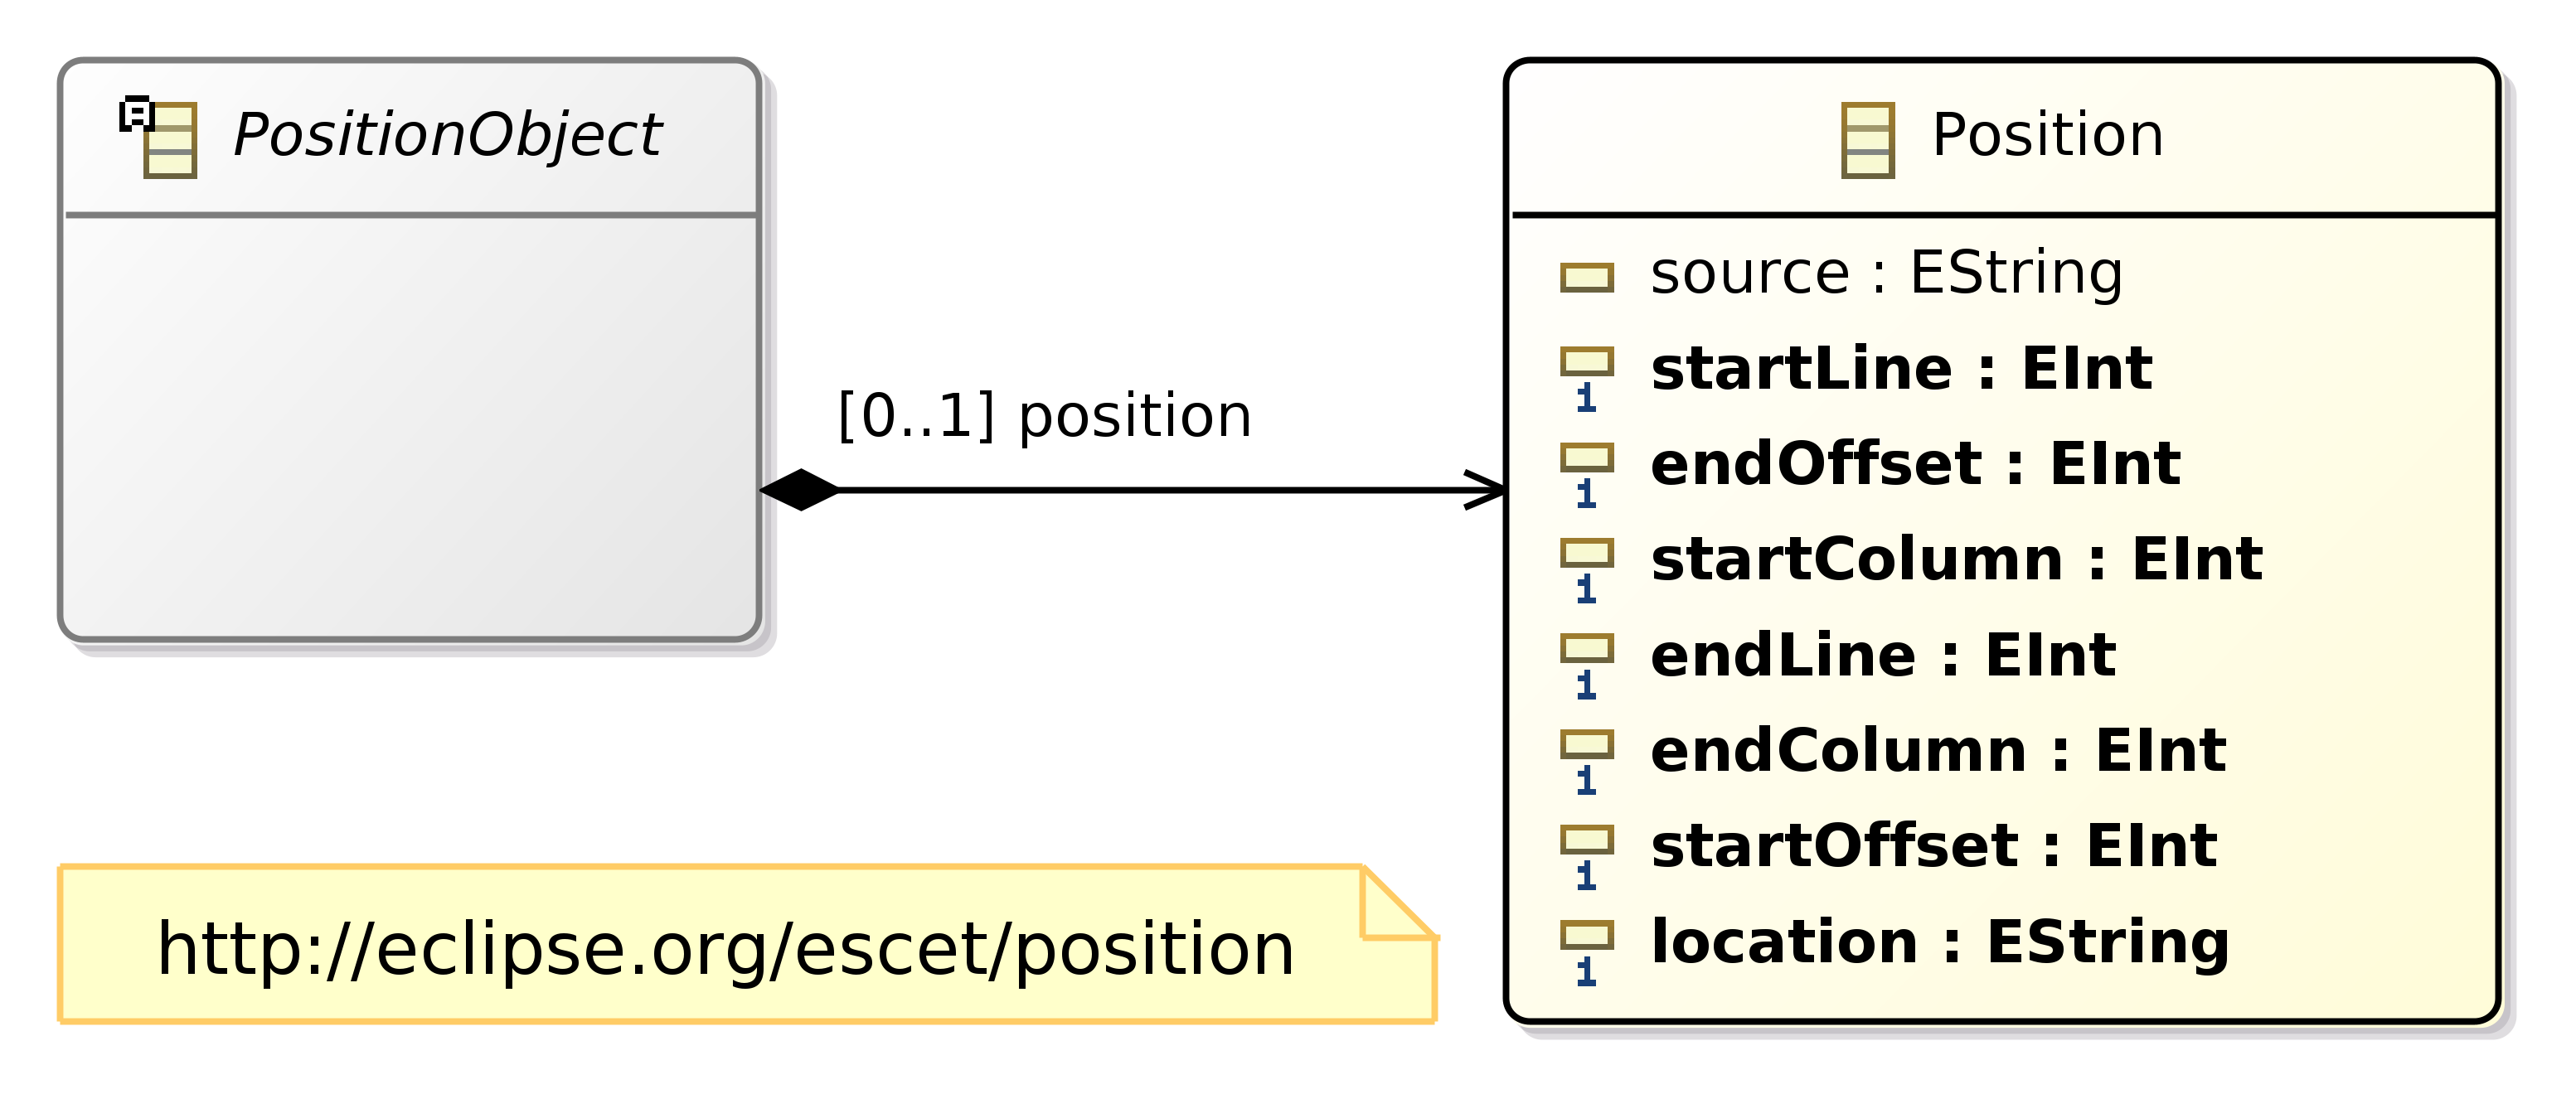
\includegraphics[width=\textwidth]{../model/position.png}
  \caption{\textit{position} package}\label{fig:pkg:position}
\end{figure}

The position package contains classes used to represent position information,
for source tracking. A position is represented as a continuous region in a
textual source (the \emph{source text}).

The \positionclass{Position} class represents actual position information.
The abstract \positionclass{PositionObject} class can be used as a base class
for other classes, and allows those classes to store position information.
}

% Position (class)
\newcommand{\clsdocuPosition}{
Position (source tracking) information.

\begin{constraints}
\citem{Position.lines}
  The \texttt{startLine} must be smaller than or equal to the \texttt{endLine}.
\citem{Position.columns}
  If the \texttt{startLine} is equal to the \texttt{endLine}, the
  \texttt{startColumn} must be smaller than or equal to the \texttt{endColumn}.
\citem{Position.offsets}
  The \texttt{startOffset} must be smaller than or equal to the
  \texttt{endOffset}.
\end{constraints}
}

\newcommand{\featdocuPositionendColumn}{
The 1-based column index of the end (inclusive) of the position region, with
respect to the start of the source text.

\begin{constraints}
\citem{Position.endColumnValue}
  Value must be greater than or equal to one.
\end{constraints}
}

\newcommand{\featdocuPositionendLine}{
The 1-based line index of the end (inclusive) of the position region, with
respect to the start of the source text.

\begin{constraints}
\citem{Position.endLineValue}
  Value must be greater than or equal to one.
\end{constraints}
}

\newcommand{\featdocuPositionendOffset}{
The 0-based byte index of the end (inclusive) of the position region, with
respect to the start of the source text.

\begin{constraints}
\citem{Position.endOffsetValue}
  Value must be greater than or equal to zero.
\end{constraints}
}

\newcommand{\featdocuPositionlocation}{
The location of the source file that contains the position. Must be an absolute
local file system path, with platform specific path separators. The path does
not have to refer to an existing file. That is, it may not be assumed that a
file with that path actually exists on disk.
}

\newcommand{\featdocuPositionsource}{
Optional source identification. Usually, this is a file name.
}

\newcommand{\featdocuPositionstartColumn}{
The 1-based column index of the start (inclusive) of the position region, with
respect to the start of the source text.

\begin{constraints}
\citem{Position.startColumnValue}
  Value must be greater than or equal to one.
\end{constraints}
}

\newcommand{\featdocuPositionstartLine}{
The 1-based line index of the start (inclusive) of the position region, with
respect to the start of the source text.

\begin{constraints}
\citem{Position.startLineValue}
  Value must be greater than or equal to one.
\end{constraints}
}

\newcommand{\featdocuPositionstartOffset}{
The 0-based byte index of the start (inclusive) of the position region,
with respect to the start of the source text.

\begin{constraints}
\citem{Position.startOffsetValue}
  Value must be greater than or equal to zero.
\end{constraints}
}

% PositionObject (abstract class)
\newcommand{\clsdocuPositionObject}{
Base class for other classes, facilitating the storage of position information.
}

\newcommand{\featdocuPositionObjectposition}{
Optional position information.
}

%%%%%%%%%%%%%%%%%%%%%%%%%%%%%%%%%%%%%%%%%%%%%%%%%%%%%%%%%%%%%%%%%%%%%%%%%%%%%%%
%% Copyright (c) 2010, 2021 Contributors to the Eclipse Foundation
%%
%% See the NOTICE file(s) distributed with this work for additional
%% information regarding copyright ownership.
%%
%% This program and the accompanying materials are made available under the terms
%% of the MIT License which is available at https://opensource.org/licenses/MIT
%%
%% SPDX-License-Identifier: MIT
%%%%%%%%%%%%%%%%%%%%%%%%%%%%%%%%%%%%%%%%%%%%%%%%%%%%%%%%%%%%%%%%%%%%%%%%%%%%%%%

%\newcommand{\positionpkg}[1]{\textit{#1} (Section~\ref{positionpkg:#1})}
%\newcommand{\positionclass}[1]{\textit{#1} (Section~\ref{positionclass:#1})}
%\newcommand{\positionattr}[1]{\textit{#1} (Section~\ref{positionattr:#1})}
%\newcommand{\positionenumlit}[1]{\textit{#1} (Section~\ref{positionenumlit:#1})}
%\newcommand{\positionclassDetail}[7]{\item {#1} \textbf{#2} {#3} :
%    {\textit{#4}} {#5} {#6} \hfill \\ {#7}}
%\newcommand{\positionenumlitDetail}[4]{\item literal \textbf{#1} {#2} {#3}
%    \hfill \\ {#4}}
%\newcommand{\hook}{\hspace*{5pt}\raisebox{2.5pt}{$\llcorner$}}
%\newcommand{\hookindent}{\hspace*{15pt}}

\section{Package position}\label{positionpkg:position}
\pkgdocuposition

\begin{description}
\item[Package URI] http://eclipse.org/escet/position
\item[Namespace prefix] position
\item[Sub-packages] none
\end{description}

\subsection{Position (class)}\label{positionclass:Position}
\clsdocuPosition

~\\ \noindent \emph{EObject} \\
\hook~\emph{Position}

~\\ \noindent Direct derived classes:
none

\begin{description}
\positionclassDetail{attr}{endColumn}{{[1]}}{EInt}{}{\label{positionattr:Position.endColumn}}
{\featdocuPositionendColumn}
\positionclassDetail{attr}{endLine}{{[1]}}{EInt}{}{\label{positionattr:Position.endLine}}
{\featdocuPositionendLine}
\positionclassDetail{attr}{endOffset}{{[1]}}{EInt}{}{\label{positionattr:Position.endOffset}}
{\featdocuPositionendOffset}
\positionclassDetail{attr}{location}{{[1]}}{EString}{}{\label{positionattr:Position.location}}
{\featdocuPositionlocation}
\positionclassDetail{attr}{source}{{[0..1]}}{EString}{}{\label{positionattr:Position.source}}
{\featdocuPositionsource}
\positionclassDetail{attr}{startColumn}{{[1]}}{EInt}{}{\label{positionattr:Position.startColumn}}
{\featdocuPositionstartColumn}
\positionclassDetail{attr}{startLine}{{[1]}}{EInt}{}{\label{positionattr:Position.startLine}}
{\featdocuPositionstartLine}
\positionclassDetail{attr}{startOffset}{{[1]}}{EInt}{}{\label{positionattr:Position.startOffset}}
{\featdocuPositionstartOffset}
\end{description}


\subsection{PositionObject (abstract class)}\label{positionclass:PositionObject}
\clsdocuPositionObject

~\\ \noindent \emph{EObject} \\
\hook~\emph{PositionObject}

~\\ \noindent Direct derived classes:
none

\begin{description}
\positionclassDetail{cont}{position}{{[0..1]}}{Position}{}{\label{positionattr:PositionObject.position}}
{\featdocuPositionObjectposition}
\end{description}






%%%%%%%%%%%%%%%%%%%%%%%%%%%%%%%%%%%%%%%%%%%%%%%%%%%%%%%%%%%%%%%%%%%%%%%%%%%%%%%
\chapter{Legal}

The material in this documentation is
Copyright (c) 2010, 2020 Contributors to the Eclipse Foundation.

Eclipse ESCET and ESCET are trademarks of the Eclipse Foundation.
Eclipse, and the Eclipse Logo are registered trademarks of the
Eclipse Foundation. Other names may be trademarks of their
respective owners.

\textbf{License}

The Eclipse Foundation makes available all content in this document
(``Content''). Unless otherwise indicated below, the Content is provided to you
under the terms and conditions of the MIT License. A copy of the MIT License
is available at \url{https://opensource.org/licenses/MIT}. For purposes of the
MIT License, ``Software'' will mean the Content.

If you did not receive this Content directly from the Eclipse Foundation,
the Content is being redistributed by another party (``Redistributor'') and
different terms and conditions may apply to your use of any object code in
the Content. Check the Redistributor's license that was provided with the
Content. If no such license exists, contact the Redistributor. Unless
otherwise indicated below, the terms and conditions of the MIT License
still apply to any source code in the Content and such source code may be
obtained at \url{http://www.eclipse.org}.


%%%%%%%%%%%%%%%%%%%%%%%%%%%%%%%%%%%%%%%%%%%%%%%%%%%%%%%%%%%%%%%%%%%%%%%%%%%%%%%
\addcontentsline{toc}{chapter}{Bibliography}

\bibliographystyle{plain}
\bibliography{position_ecore_doc}

\end{document}
